\documentclass{report}
\usepackage{amsmath, graphicx}
\title{Project Report\\
  Optimization Algorithms and Benchmarking}
\author{Ronit Mehta, Sajja Phani Kumar, Sayani Mondal, Swapnil Chaturvedi}
\date{}
\begin{document}
\maketitle

\section*{Project Design}
To facilitate seamless collaboration and code integration, the project architecture is modularized into three core Python files:

\begin{itemize}
    \item \texttt{algorithms.py}: Contains the \texttt{Optimization} class, which implements the unconstrained numerical optimization algorithms (Steepest Descent and Newton's Method).
    \item \texttt{test\_functions.py}: Defines a standardized class interface for each mathematical test function. Each class encapsulates its specific objective function, gradient, Hessian, and stopping criteria. This uniform structure allows the optimization algorithms to evaluate any test function dynamically without requiring changes to the core logic.
    \item \texttt{benchmarking.py}: Implements the \texttt{Benchmark} class to orchestrate the experiments. By leveraging the modular design of the test functions and optimizers, this script handles execution, performance tracking, and the generation of convergence visualizations.
\end{itemize}



\section*{Test Functions}
To evaluate the optimization algorithms across different topological landscapes, four standard two-dimensional test functions were implemented. Each function is equipped with analytical gradients and Hessians, alongside a standardized stopping criterion that halts the algorithm when the gradient norm falls below $10^{-6}$ or when $10,000$ iterations are reached.

\begin{itemize}
    \item \textbf{Sphere Function}: A strictly convex quadratic problem defined as $f(x, y) = x^2 + y^2$. It serves as a baseline for convergence testing, featuring a well-conditioned symmetric Hessian and a single global minimizer at $(0, 0)$ with $f(x^*) = 0$.
    \item \textbf{Booth Function}: A mildly ill-conditioned quadratic function defined as $f(x, y) = (x + 2y - 7)^2 + (2x + y - 5)^2$. This function tests the algorithms against differing curvature magnitudes along its axes. Its global minimum is $f(x^*) = 0$ at $(1, 3)$.
    \item \textbf{Rosenbrock Function}: A non-quadratic, non-convex function defined as $f(x, y) = 100(y - x^2)^2 + (1 - x)^2$. Often referred to as a "valley" or "banana" function, it forces the optimizer to navigate a narrow, flat valley to reach the global minimum of $f(x^*) = 0$ at $(1, 1)$. This severely tests both step-size sensitivity in steepest descent and curvature utilization in Newton's method.
    \item \textbf{Himmelblau Function}: A multimodal non-quadratic function defined as $f(x, y) = (x^2 + y - 11)^2 + (x + y^2 - 7)^2$. It features four distinct global minimizers where $f(x^*) = 0$: $(3, 2)$, $(-2.805, 3.131)$, $(-3.779, -3.283)$, and $(3.584, -1.848)$. This function is used to observe how different starting points dictate which local basin of attraction the algorithm falls into.
\end{itemize}

\section*{Testing and Benchmarking}

In this section, we present the convergence behavior of Steepest Descent and Newton's Method across our selected test functions. The performance is measured by the number of iterations required to reach the gradient norm tolerance of $10^{-6}$, the final objective value, and the final converged point.

\subsection*{1. Simple Convex Problem: Sphere Function}
To evaluate behavior on a strictly convex landscape, both algorithms were initialized at $x_0 = (5.0, 5.0)$. To analyze the effect of step size on Steepest Descent, multiple fixed step sizes were evaluated, including the default optimal step size of $\alpha = 0.1$, alongside choices that demonstrate slower convergence or divergence. Using a larger step size like  $\alpha = 1.0$ results in the steepest descent method not converging in the given number of iterations.

\begin{table}[h]
\centering
\begin{tabular}{|l|c|c|c|c|}
\hline
\textbf{Method} & \textbf{Step Size} & \textbf{Iterations} & \textbf{Final $f(x)$} & \textbf{Final Point} \\ \hline

Steepest Descent & 0.1 & 74 & 2.27e-13 & (0.0000, 0.0000) \\ \hline
Steepest Descent & 0.01 & 815 & 2.50e-13 & (0.0000, 0.0000) \\ \hline
Steepest Descent & 0.9 & 74 & 2.27e-13 & (0.0000, 0.0000) \\ \hline
Newton's Method & N/A & 1 & 0.00 & (0.0000, 0.0000) \\ \hline
\end{tabular}
\caption{Benchmarking results for the Sphere Function.}
\end{table}

\textbf{Interpretation:} The medium and small step sizes result in a direct path towards the minimum, whereas the large step size results in an overshoot and a correction. The small step size results in a large amout of iterations. The newton method converges with just 1 iteration.

\begin{figure}[h]
    \centering

    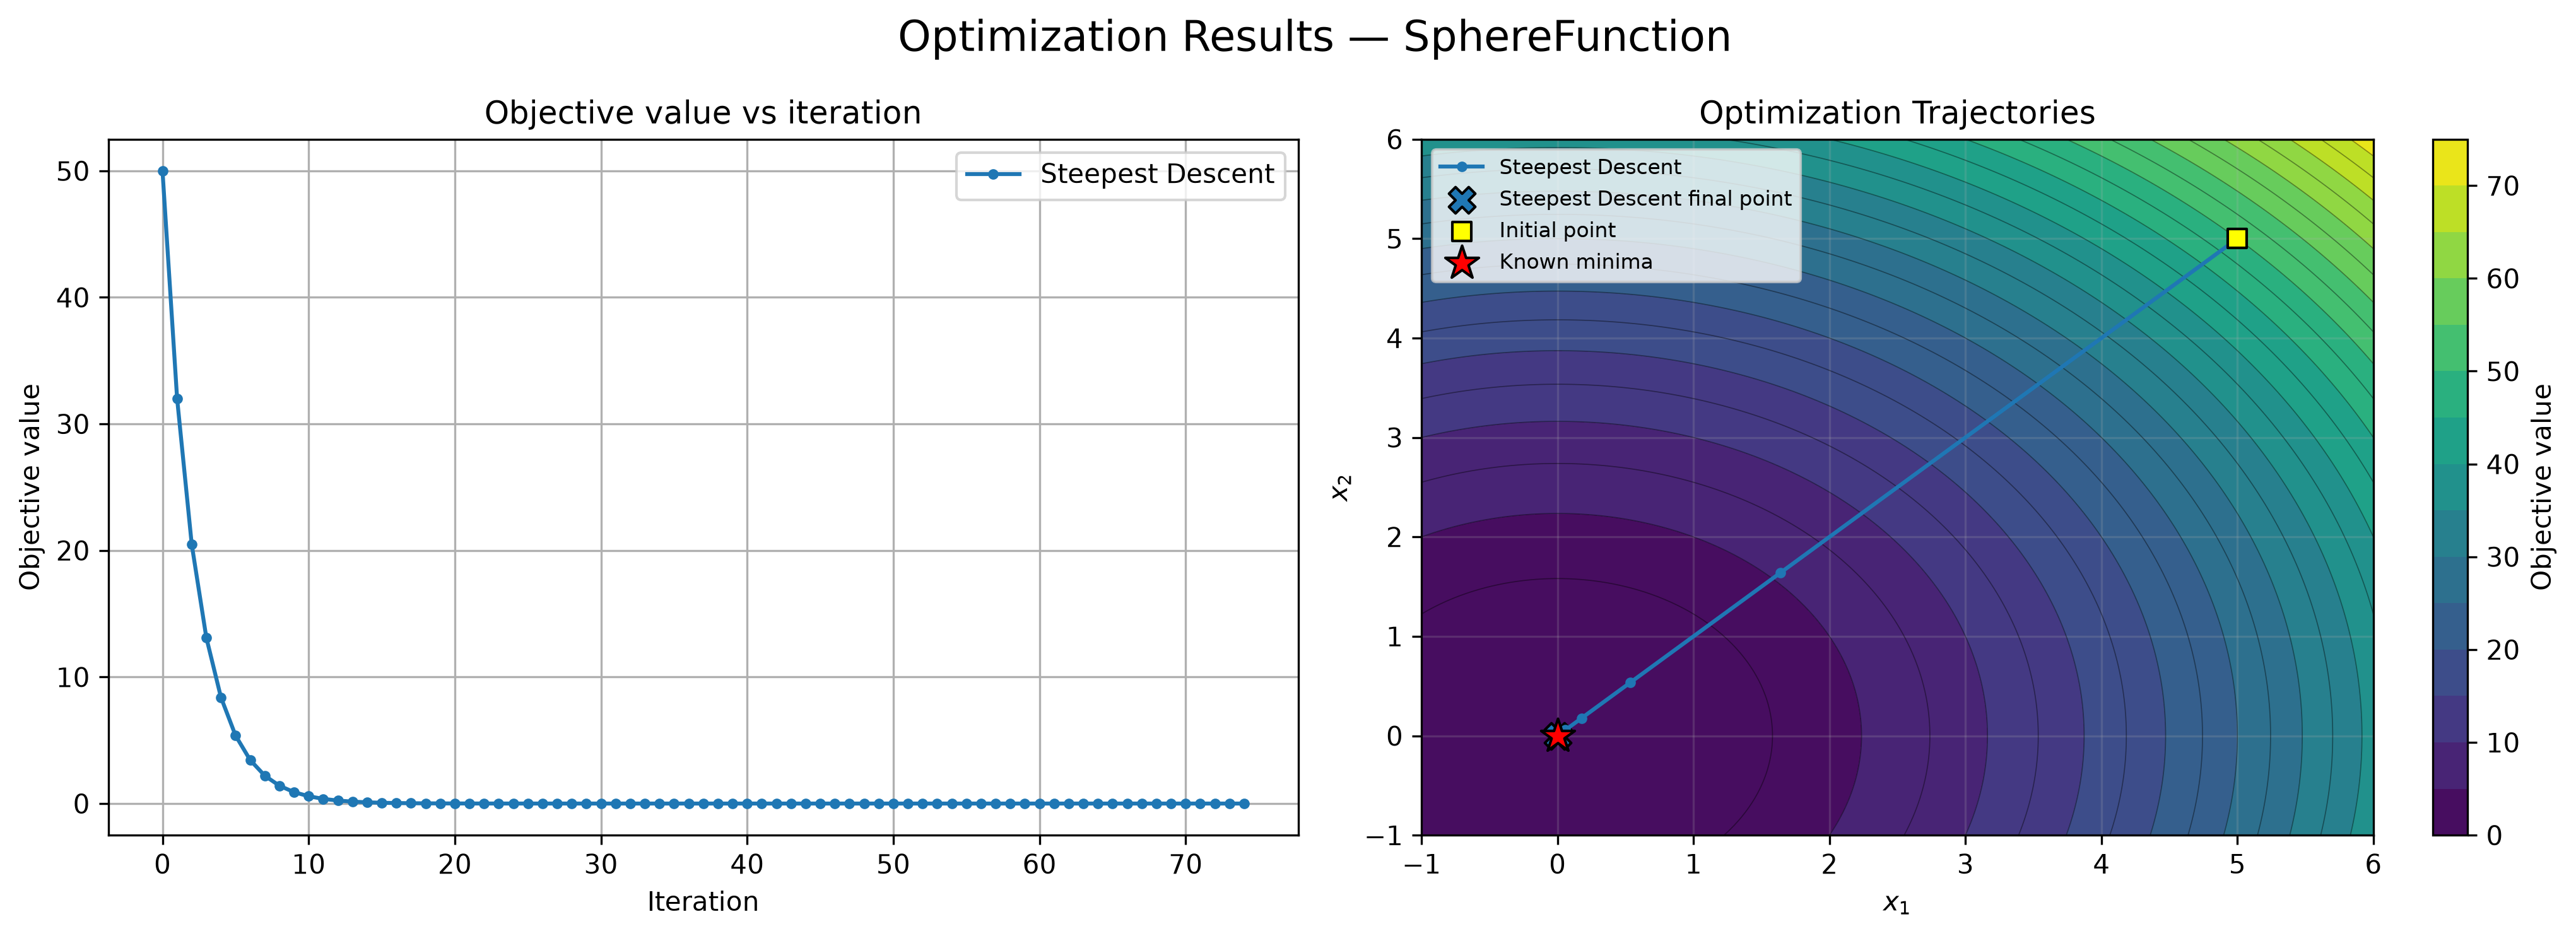
\includegraphics[width=0.45\textwidth]{sphere_steepest_med.png}
    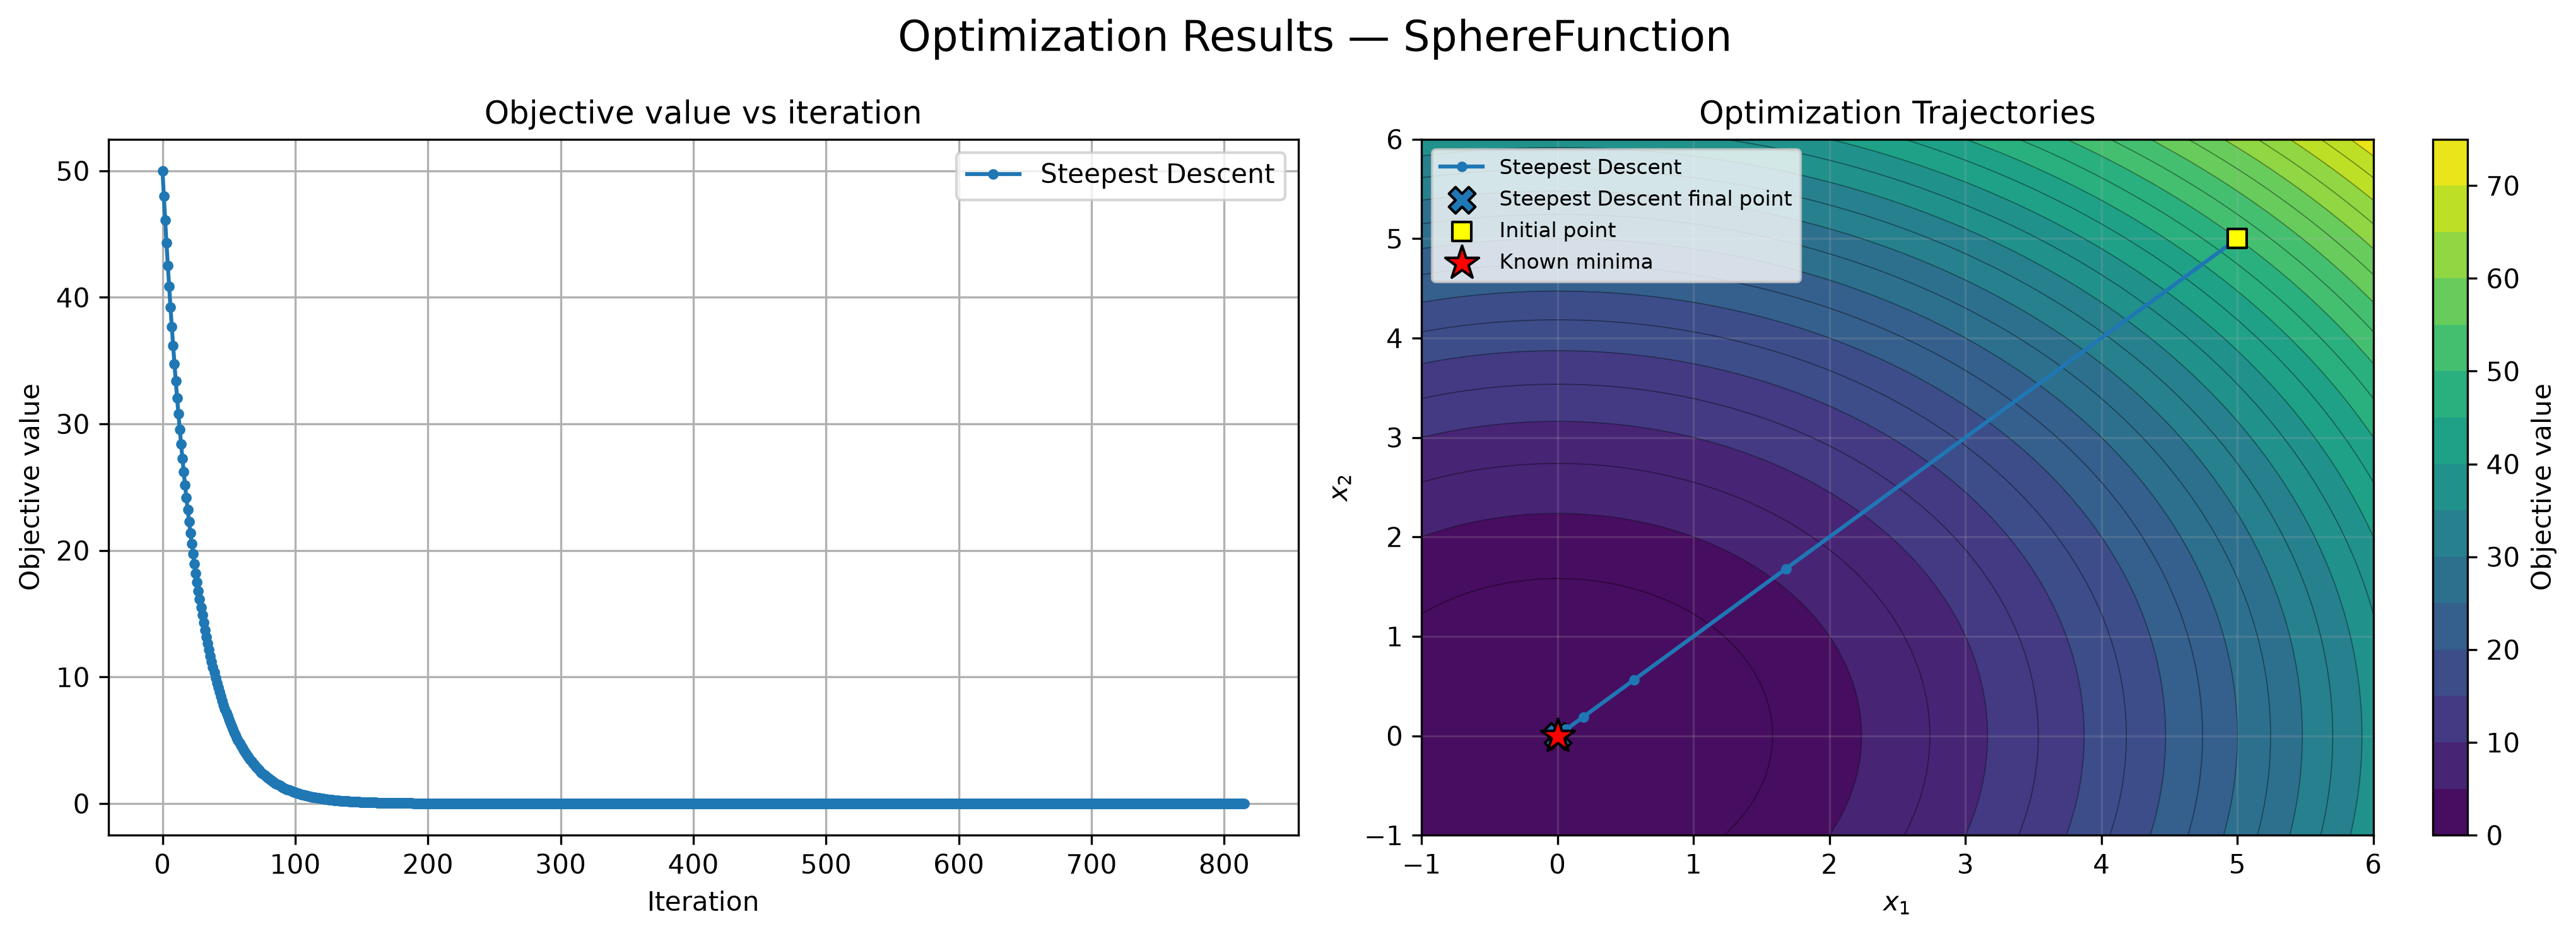
\includegraphics[width=0.45\textwidth]{sphere_steepest_small.png}
    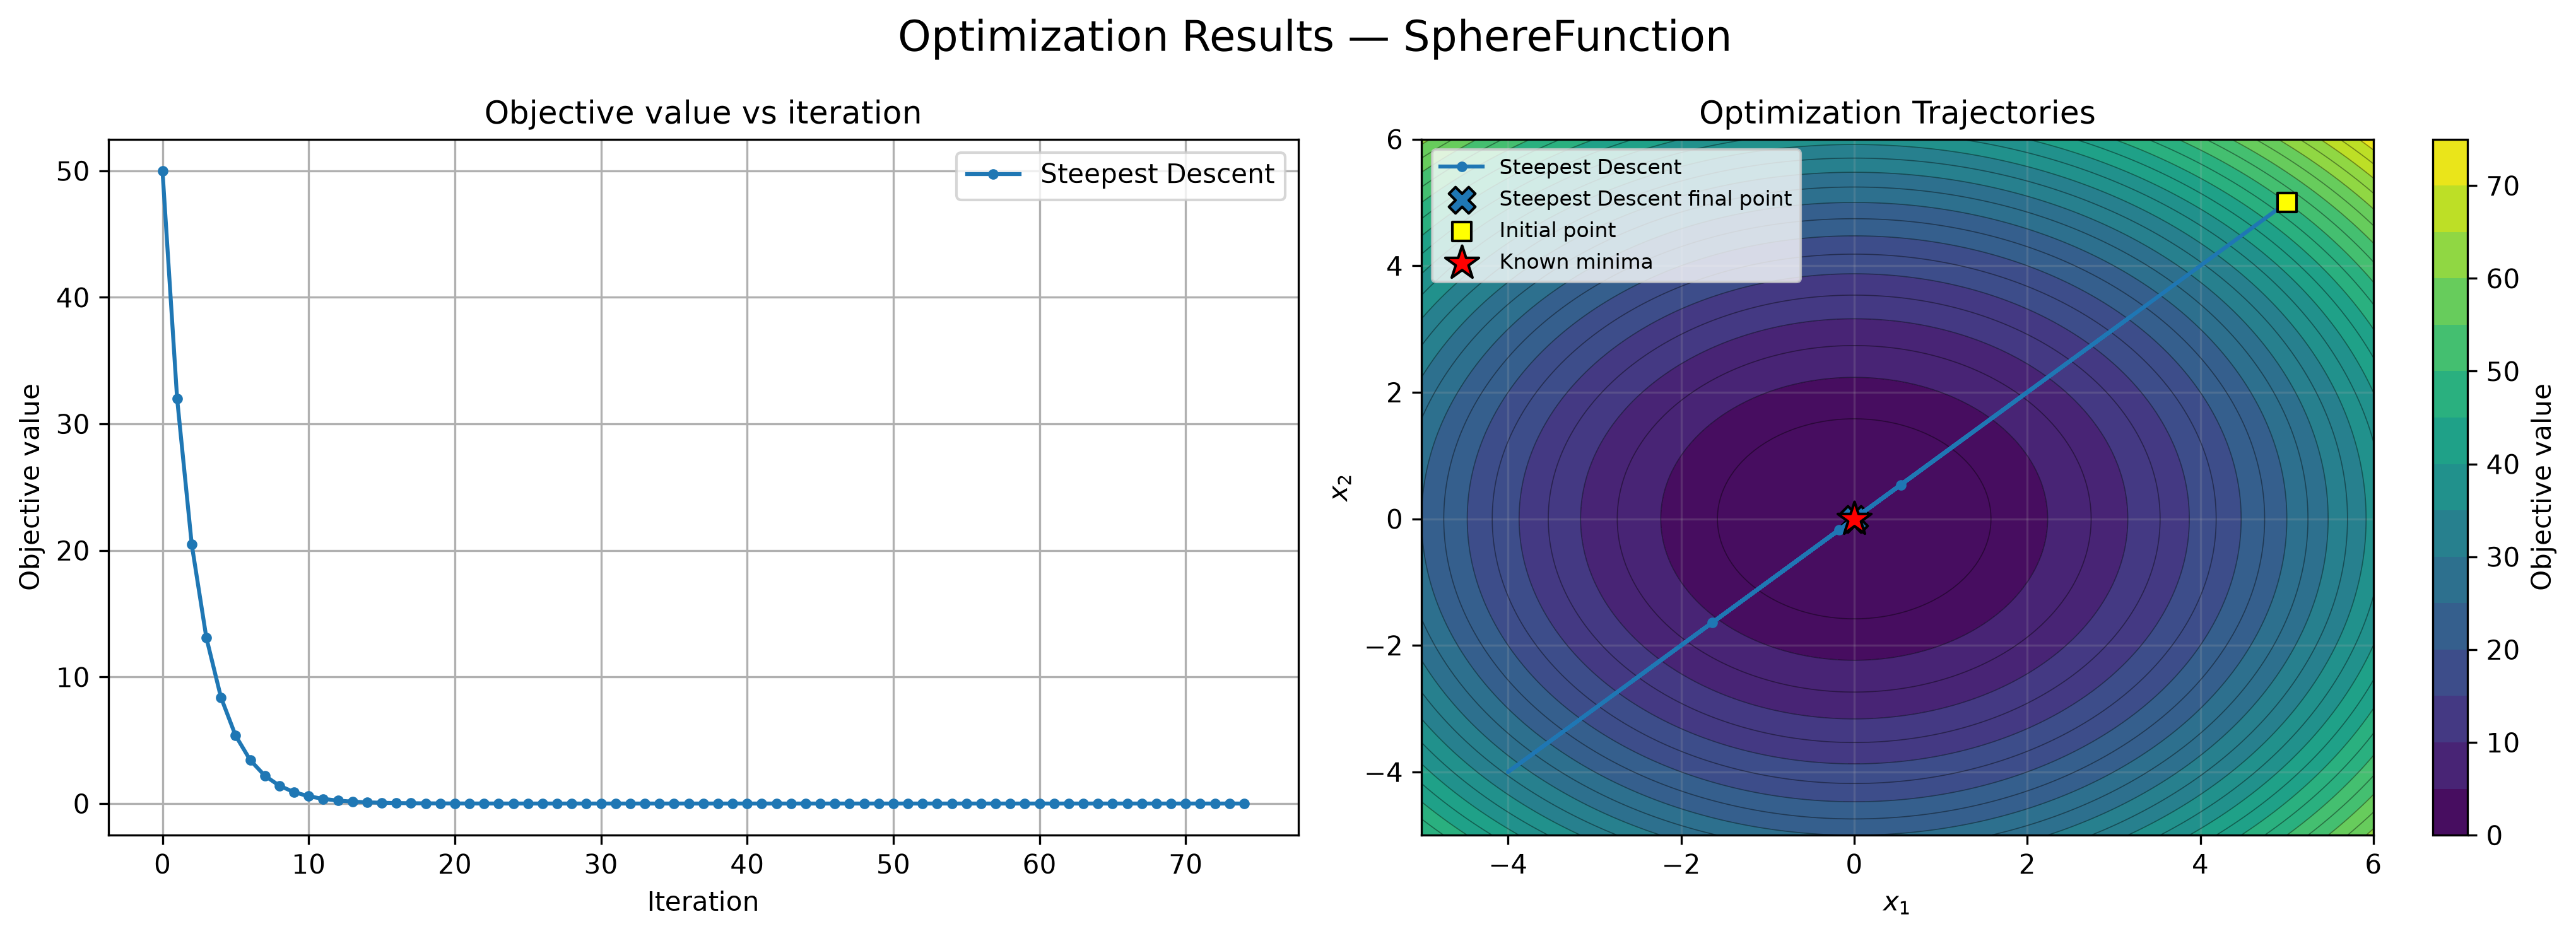
\includegraphics[width=0.45\textwidth]{sphere_steepest_large.png}
    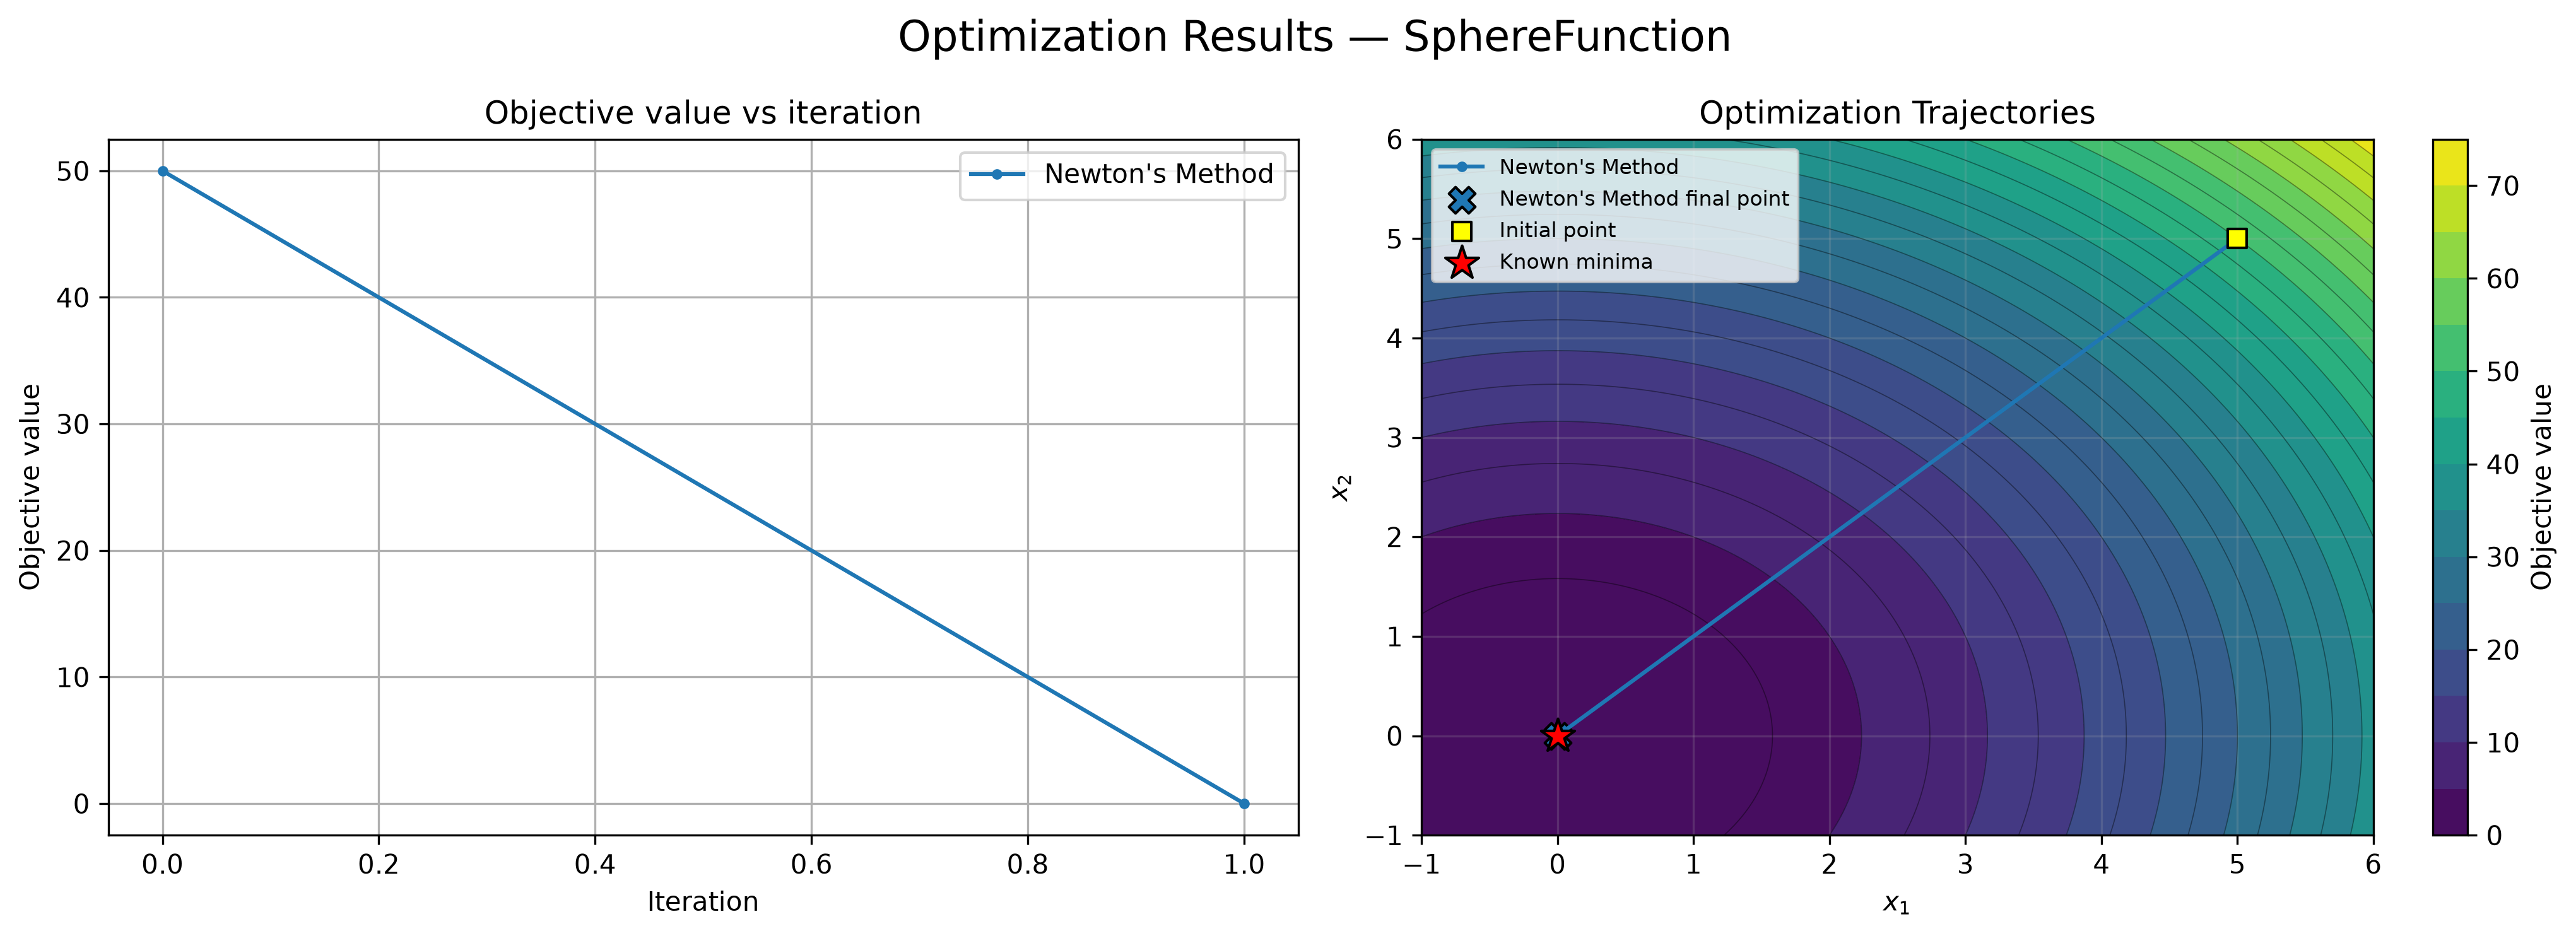
\includegraphics[width=0.45\textwidth]{sphere_newton.png}
    
    \caption{Convergence trajectories and objective value decay for the Sphere Function. Top: medium and small step size steepest descent, Bottom-Left: large step size, Bottom-right: newton method}
\end{figure}

\subsection*{2. Ill-Conditioned Quadratic: Booth Function}
To observe how conditioning affects the optimization path, both algorithms were evaluated on the Booth function starting at $x_0 = (0.0, 0.0)$. The Steepest Descent method utilized a step size of $\alpha = 0.01$.

\begin{table}[h]
\centering
\begin{tabular}{|l|c|c|c|}
\hline
\textbf{Method} & \textbf{Iterations} & \textbf{Final $f(x)$} & \textbf{Final Point} \\ \hline

Steepest Descent & 736 & 2.43e-13 & (1.0000, 3.0000) \\ \hline
Newton's Method & 1 & 0.00 & (1.0000, 3.0000) \\ \hline
\end{tabular}
\caption{Benchmarking results for the Booth Function.}
\end{table}

\textbf{Interpretation:} The elliptical contour lines of the Booth function indicate differing eigenvalues, which creates a mildly ill-conditioned landscape. Due to this ill-conditioning Steepest Descent has to take an indirect path to the minimizer, whereas Newton's Method utilizes the constant Hessian to perfectly scale the step to the local curvature, allowing it to shoot directly to the minimizer in a single iteration.

\begin{figure}[h]
    \centering

    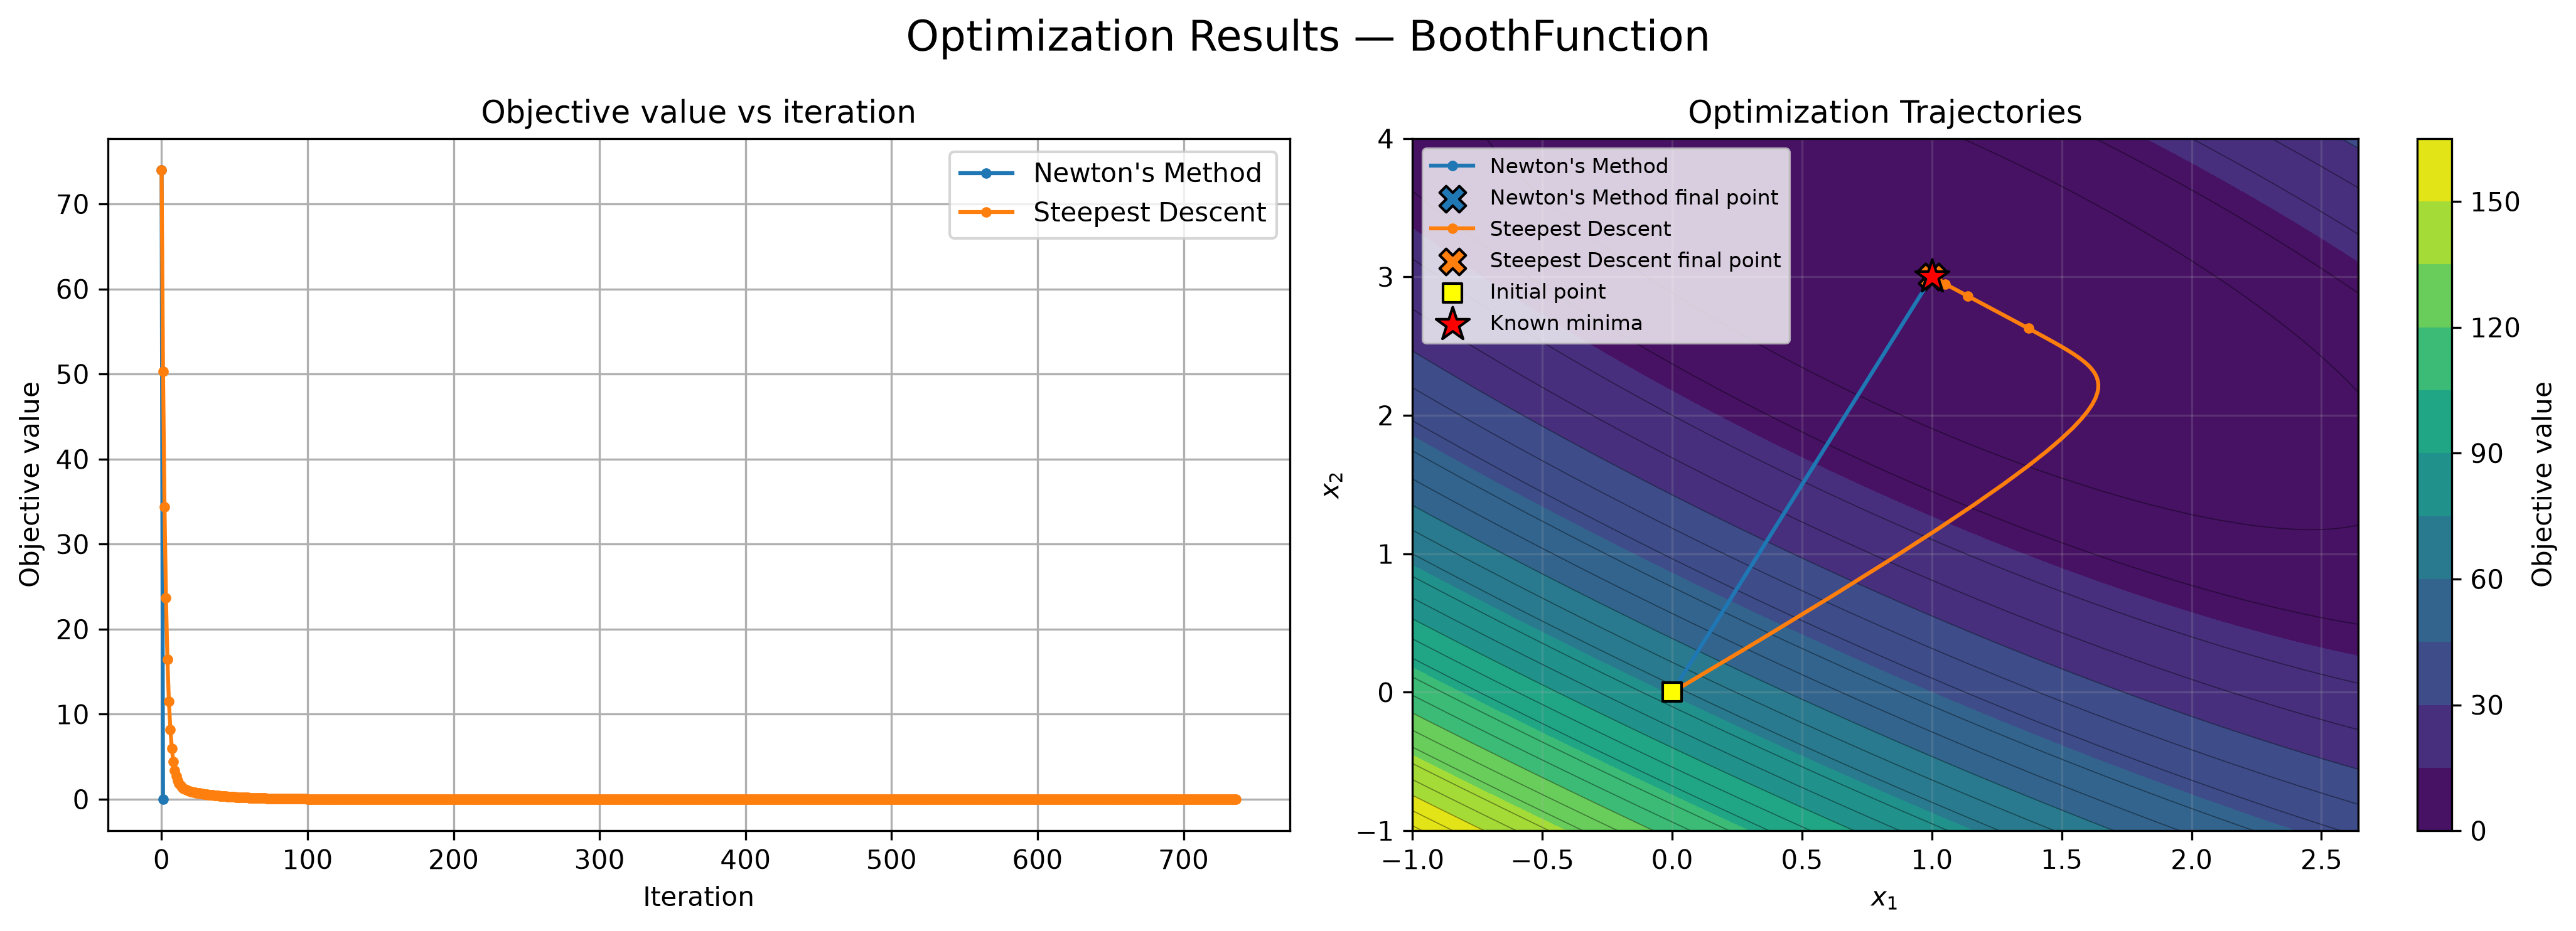
\includegraphics[width=1.2\textwidth]{booth.png}
    \caption{Convergence trajectories and objective value decay for the Booth Function.}
\end{figure}

\subsection*{3. Non-Quadratic Objective: Rosenbrock Function}
The Rosenbrock function presents a highly non-convex landscape with a narrow valley. The algorithms were tested from the standard starting point $x_0 = (-1.2, 1.0)$ using a Steepest Descent step size of $\alpha = 0.001$.

\begin{table}[h]
\centering
\begin{tabular}{|l|c|c|c|}
\hline
\textbf{Method} & \textbf{Iterations} & \textbf{Final $f(x)$} & \textbf{Final Point} \\ \hline

Steepest Descent & 10000 & 5.85e-05 & (0.9924, 0.9847) \\ \hline
Newton's Method & 6 & 3.43e-20 & (1.0000, 1.0000) \\ \hline

\end{tabular}
\caption{Benchmarking results for the Rosenbrock Function.}
\end{table}

\textbf{Interpretation:} The Rosenbrock function features a notoriously flat, parabolic valley. As shown in the optimization trajectories, Steepest Descent rapidly descends into the valley but then severely struggles to navigate the flat floor, ultimately failing to reach the gradient tolerance within the 10,000 maximum iteration limit (halting at an objective value of $5.85 \times 10^{-5}$). Newton's Method easily overcomes this by incorporating second-order derivative information, allowing it to scale the local curvature and take aggressive, accurate steps to find the exact minimum at (1.0000, 1.0000) in just 6 iterations. 

\begin{figure}[h]
    \centering

    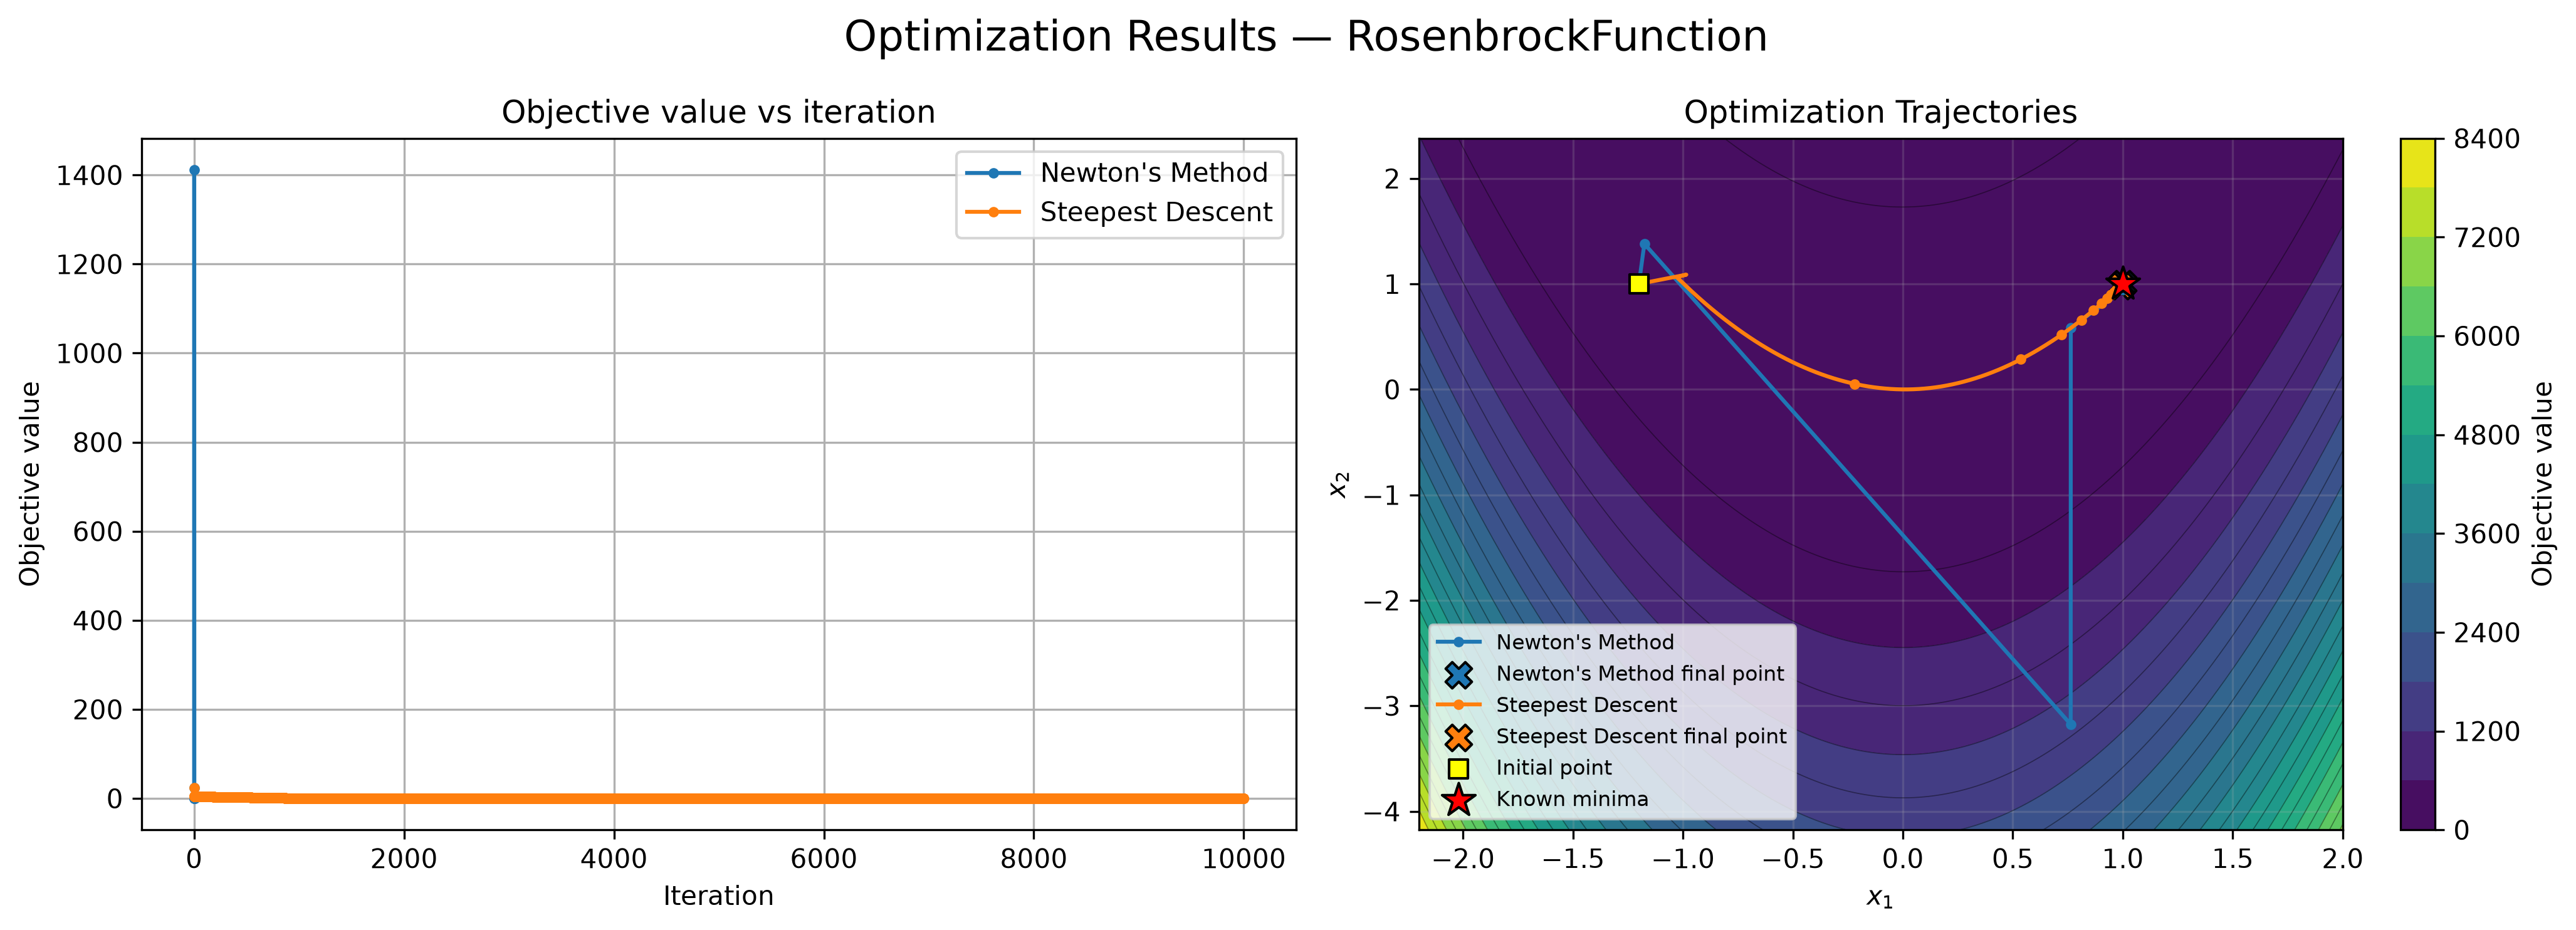
\includegraphics[width=1.2\textwidth]{rosenbrock.png}
    \caption{Convergence trajectories and objective value decay for the Rosenbrock Function.}
\end{figure}

\subsection*{4. Multimodal Objective: Himmelblau Function}
The Himmelblau function tests the algorithms' convergence to one of four global minima. The initial starting point evaluated is $x_0 = (0.0, 0.0)$, using a Steepest Descent step size of $\alpha = 0.001$.

\begin{table}[h]
\centering
\begin{tabular}{|l|c|c|c|}
\hline
\textbf{Method} & \textbf{Iterations} & \textbf{Final $f(x)$} & \textbf{Final Point} \\ \hline

Steepest Descent & 672 & 1.91e-14 & (3.0000, 2.0000) \\ \hline
Newton's Method & 67 & 2.49e-22 & (3.5844, -1.8481) \\ \hline
\end{tabular}
\caption{Benchmarking results for the Himmelblau Function.}
\end{table}

\textbf{Interpretation:} Because the Himmelblau function has multiple global minima, the choice of algorithm from the exact same starting point $(0,0)$ dictated which basin of attraction the optimizer fell into. Steepest Descent smoothly followed the immediate local gradient path upwards, converging to the minimizer at (3.0000, 2.0000) after 672 iterations. Newton's Method, taking much larger initial steps dictated by the local curvature matrix, jumped across the landscape to converge at a completely different minimizer at (3.5844, -1.8481) in only 67 iterations.

\begin{figure}[h]
    \centering
    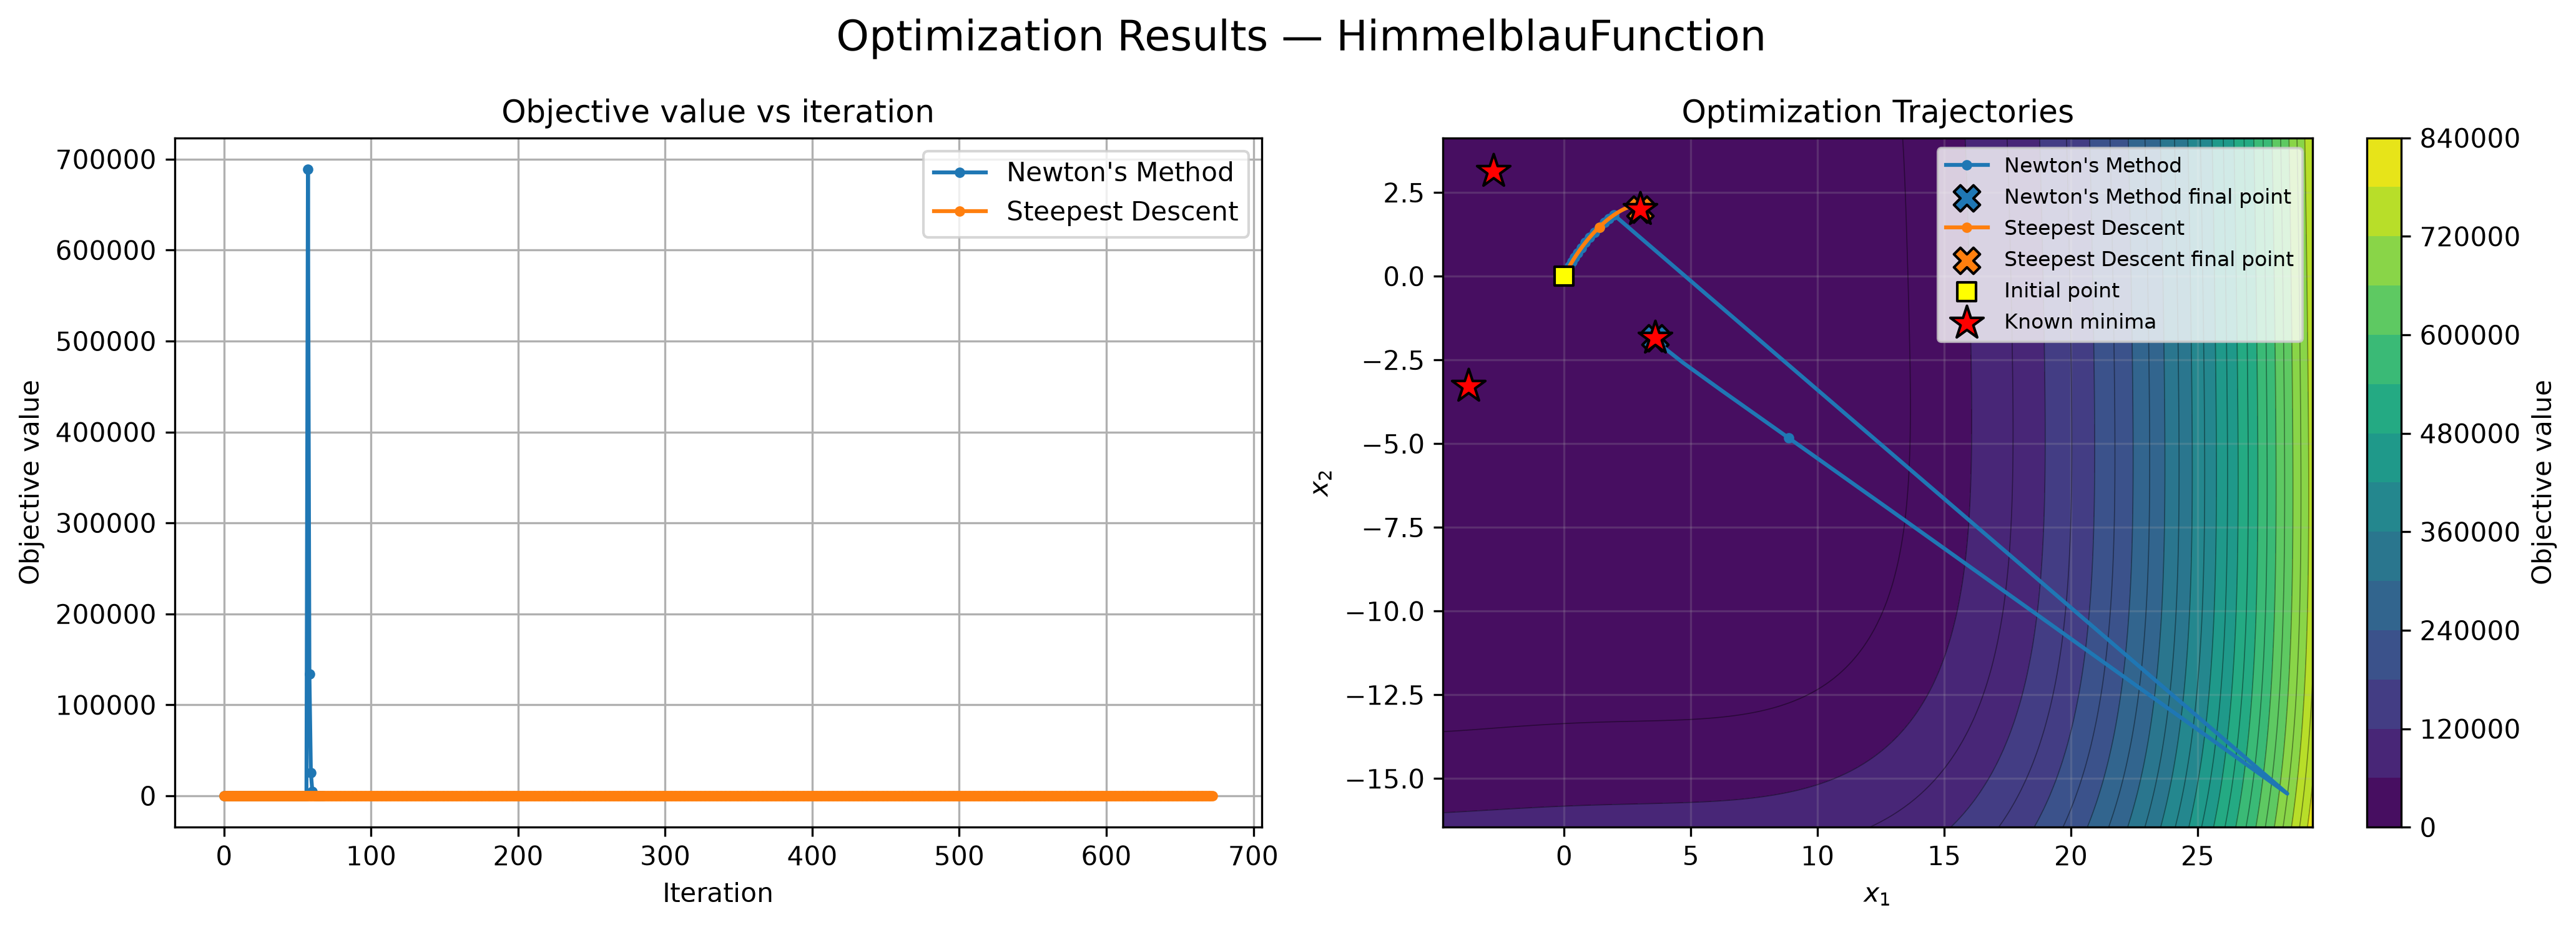
\includegraphics[width=1.2\textwidth]{himmelblau.png}
    \caption{Convergence trajectories and objective value decay for the Himmelblau Function.}
\end{figure}
\end{document}
